\documentclass[border=10pt]{standalone}
\usepackage[svgnames]{xcolor}
\usepackage{amsmath}
\usepackage{pgfplots}
\pgfplotsset{compat=newest}
\usepackage[sfdefault]{FiraSans}
\usepackage{FiraMono}
\renewcommand*\familydefault{\sfdefault}
\begin{document}
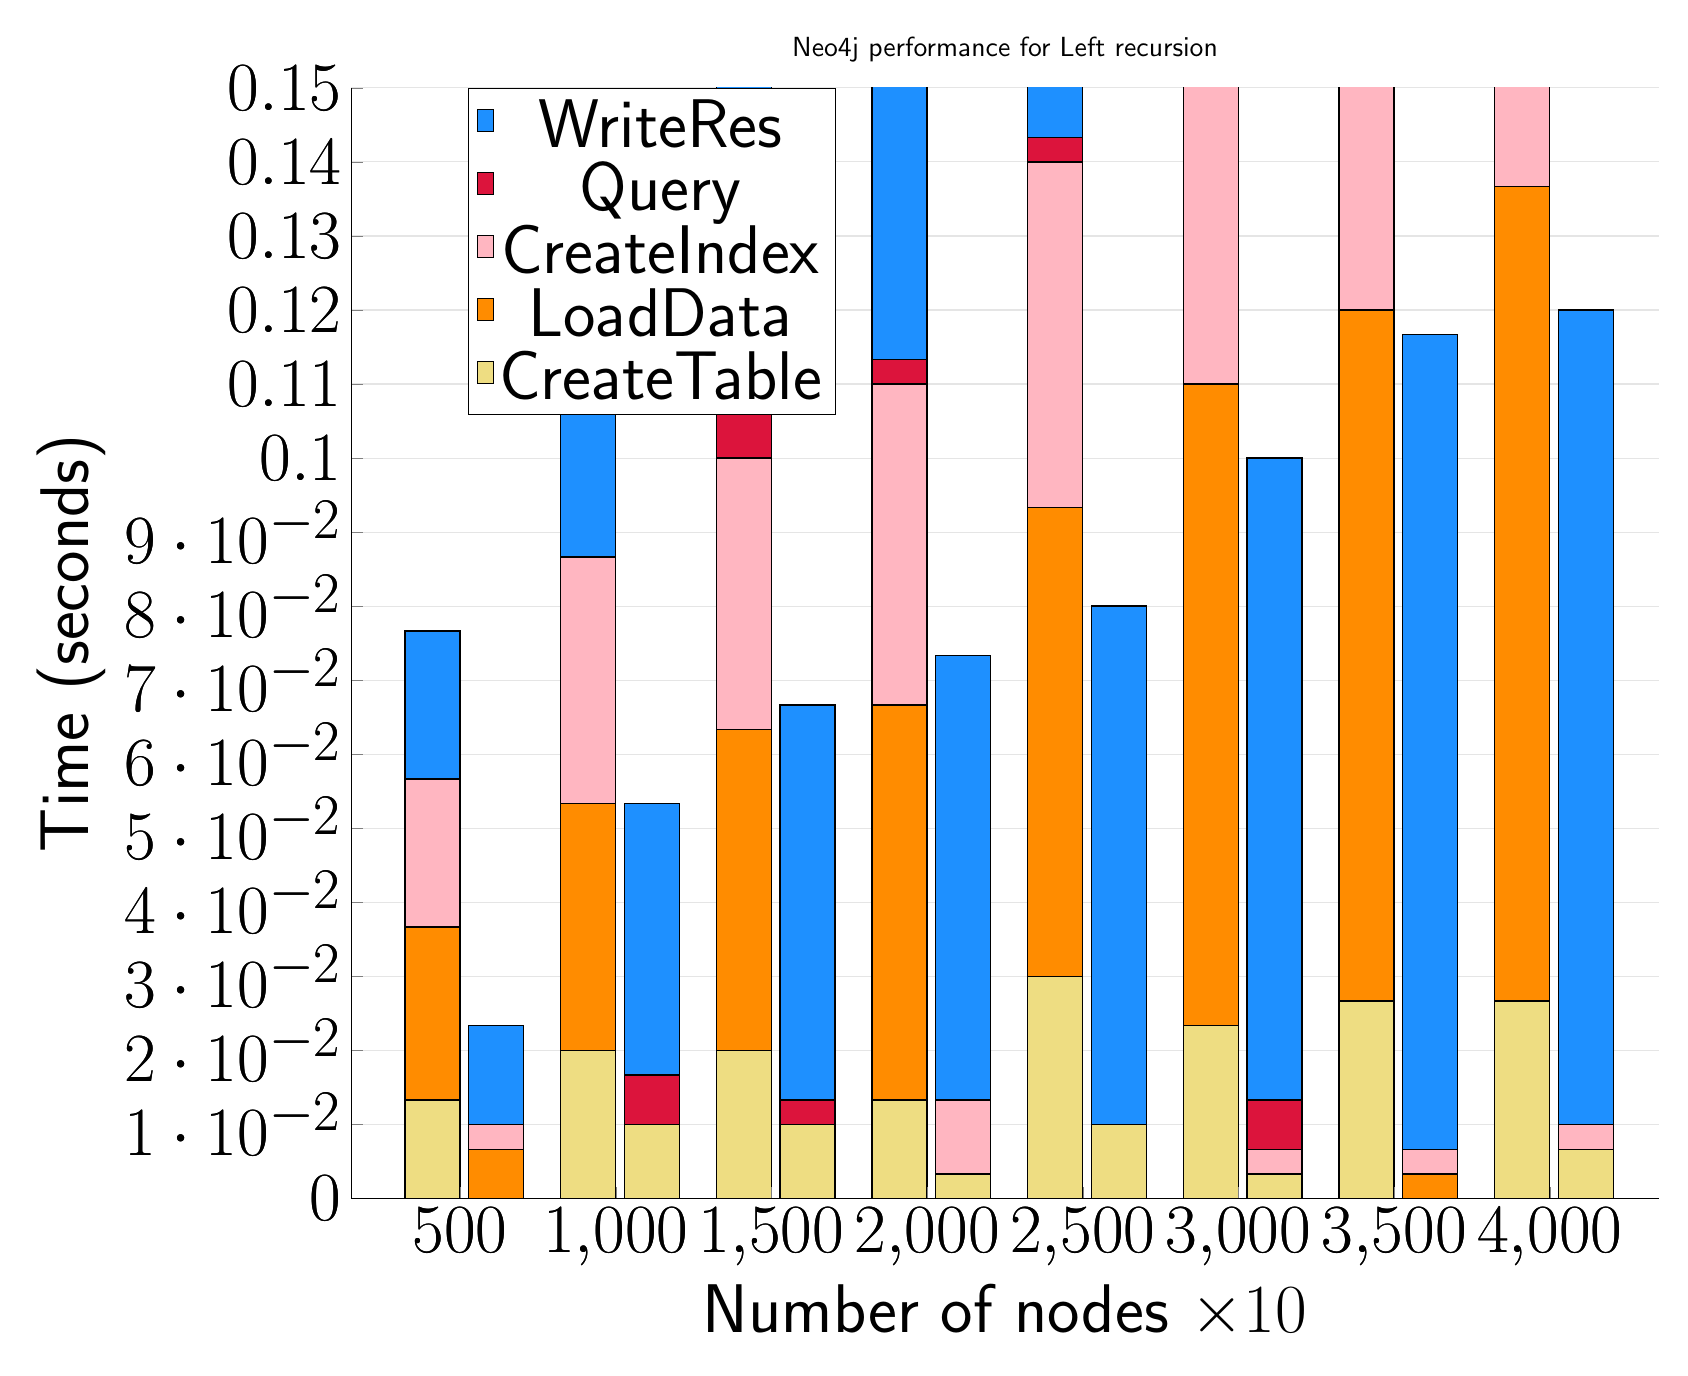
\begin{tikzpicture}
\begin{axis}[
   ybar stacked,
   title={Neo4j performance for Left recursion},
   bar shift=-10pt,
   width=1.5\textwidth,
   bar width=0.7cm,
   ymajorgrids, tick align=inside,
   major grid style={draw=gray!20},
   xtick=data,
   ymin=0, ymax=0.15000000019868215,
   axis x line*=bottom,
   axis y line*=left,
   enlarge x limits=0.1,
   legend style={
       at={(0.23, 1)},
       anchor=north,
       legend columns=1,
       font=\Huge,
   },
   ylabel={Time (seconds)},
   xlabel={Number of nodes $\times 10$},
   label style={font=\Huge},
   tick label style={font=\Huge},
]
\addlegendimage{fill=DodgerBlue, draw=black, line width=0.2pt}
\addlegendentry{WriteRes}
\addlegendimage{fill=Crimson, draw=black, line width=0.2pt}
\addlegendentry{Query}
\addlegendimage{fill=LightPink, draw=black, line width=0.2pt}
\addlegendentry{CreateIndex}
\addlegendimage{fill=DarkOrange, draw=black, line width=0.2pt}
\addlegendentry{LoadData}
\addlegendimage{fill=LightGoldenrod, draw=black, line width=0.2pt}
\addlegendentry{CreateTable}
\addplot +[fill=LightGoldenrod, draw=black, line width=0.5pt] coordinates {
    (500, 0.013333335518836975)
    (1000, 0.020000000794728596)
    (1500, 0.020000000794728596)
    (2000, 0.01333333303531011)
    (2500, 0.030000001192092896)
    (3000, 0.023333333432674408)
    (3500, 0.02666666607062022)
    (4000, 0.02666666607062022)
};
\addplot +[fill=DarkOrange, draw=black, line width=0.5pt] coordinates {
    (500, 0.023333333432674408)
    (1000, 0.033333333830038704)
    (1500, 0.04333333174387614)
    (2000, 0.05333333214124044)
    (2500, 0.06333333005507787)
    (3000, 0.08666666597127914)
    (3500, 0.09333333373069763)
    (4000, 0.10999999940395355)
};
\addplot +[fill=LightPink, draw=black, line width=0.5pt] coordinates {
    (500, 0.019999998311201733)
    (1000, 0.03333333383003871)
    (1500, 0.03666666895151138)
    (2000, 0.04333333174387614)
    (2500, 0.04666666934887568)
    (3000, 0.05999999990065892)
    (3500, 0.07333333293596904)
    (4000, 0.07666666557391486)
};
\addplot +[fill=Crimson, draw=black, line width=0.5pt] coordinates {
    (500, 0.0)
    (1000, 0.0)
    (1500, 0.019999998311201733)
    (2000, 0.003333332637945811)
    (2500, 0.003333332637945811)
    (3000, 0.0066666677594184875)
    (3500, 0.0)
    (4000, 0.0)
};
\addplot +[fill=DodgerBlue, draw=black, line width=0.5pt] coordinates {
    (500, 0.020000000794728596)
    (1000, 0.04333333174387614)
    (1500, 0.06000000238418579)
    (2000, 0.06666666766007741)
    (2500, 0.08000000069538753)
    (3000, 0.10666666676600774)
    (3500, 0.13000000019868216)
    (4000, 0.12999999771515527)
};
\end{axis}
\begin{axis}[
   ybar stacked,
   bar shift=13pt,
   width=1.5\textwidth,
   bar width=0.7cm,
   ymajorgrids, tick align=inside,
   major grid style={draw=none},
   xtick=data,
   ymin=0, ymax=0.15000000019868215,
   axis x line*=none,
   axis y line*=none,
   enlarge x limits=0.1,
   label style={font=\Huge},
   tick label style={font=\Huge},
]
\addplot +[fill=LightGoldenrod, draw=black, line width=0.5pt] coordinates {
    (500, 0.0)
    (1000, 0.010000000000000004)
    (1500, 0.010000000000000005)
    (2000, 0.0033333333333333375)
    (2500, 0.010000000000000009)
    (3000, 0.003333333333333337)
    (3500, 0.0)
    (4000, 0.006666666666666654)
};
\addplot +[fill=DarkOrange, draw=black, line width=0.5pt] coordinates {
    (500, 0.006666666666666675)
    (1000, 0.0)
    (1500, 0.0)
    (2000, 0.0)
    (2500, 0.0)
    (3000, 0.0)
    (3500, 0.003333333333333336)
    (4000, 0.0)
};
\addplot +[fill=LightPink, draw=black, line width=0.5pt] coordinates {
    (500, 0.0033333333333333184)
    (1000, 0.0)
    (1500, 0.0)
    (2000, 0.010000000000000004)
    (2500, 0.0)
    (3000, 0.003333333333333318)
    (3500, 0.003333333333333337)
    (4000, 0.003333333333333336)
};
\addplot +[fill=Crimson, draw=black, line width=0.5pt] coordinates {
    (500, 0.0)
    (1000, 0.006666666666666674)
    (1500, 0.003333333333333332)
    (2000, 0.0)
    (2500, 0.0)
    (3000, 0.00666666666666665)
    (3500, 0.0)
    (4000, 0.0)
};
\addplot +[fill=DodgerBlue, draw=black, line width=0.5pt] coordinates {
    (500, 0.01333333333333333)
    (1000, 0.03666666666666663)
    (1500, 0.05333333333333332)
    (2000, 0.06)
    (2500, 0.06999999999999999)
    (3000, 0.08666666666666667)
    (3500, 0.11000000000000003)
    (4000, 0.11000000000000003)
};
\end{axis}
\end{tikzpicture}

\end{document}
